\documentclass[a4paper, 12pt, notitlepage]{article}
\title{Bài tập tuần 1}
\author{Tạ Chí Thành Danh}
\usepackage[utf8]{vietnam} % Unicode tiếng Việt
\usepackage[left=1.5cm,right=2cm,top=2cm,bottom=2cm]{geometry} % Định dạng khoảng cách lề giấy
\usepackage{enumitem} % https://tex.stackexchange.com/questions/116101/add-bold-enumerate-items
% \setlist[enumerate]{font=\bfseries}
\usepackage{graphicx} % https://latex-tutorial.com/tutorials/figures/
\begin{document}
	\maketitle
	\begin{enumerate}[font=\bfseries]
		\item[1.2]
		\begin{enumerate}
			\item Chương trình in dòng chữ \verb|Hello World| ra màn hình
			\item Thay chữ \verb|Hello World| trong chương trình bằng chữ \verb|Chao mung|, chạy lại chương trình, chương trình in dòng chữ \verb|Chao mung| ra màn hình thay vì dòng chữ \verb|Hello World|
		\end{enumerate}
		\item[1.3] Chương trình yêu cầu nhập 3 biến \verb|a|, \verb|b|, \verb|c| và xuất giá trị lớn nhất ra màn hình (giá trị này được lưu trong biến \verb|max|) 
		\item[1.4] Chương trình yêu cầu nhập biến \verb|n| và xuất tích các số nguyên từ $1$ đến $n$ thông qua biến \verb|s|
		\item[1.5] 
		\begin{enumerate}
			\item Khi chương trình thực hiện \verb|max| lần lượt nhận các giá trị: \verb|1, 5|
			\item Nhập \verb|n = 10|, khi \verb|n = 3| thì \verb|s = 1814400|
		\end{enumerate} 
	\end{enumerate}
	Hình ảnh minh chứng cho từng bài tập:
	\begin{figure}[h]
		\begin{center}
			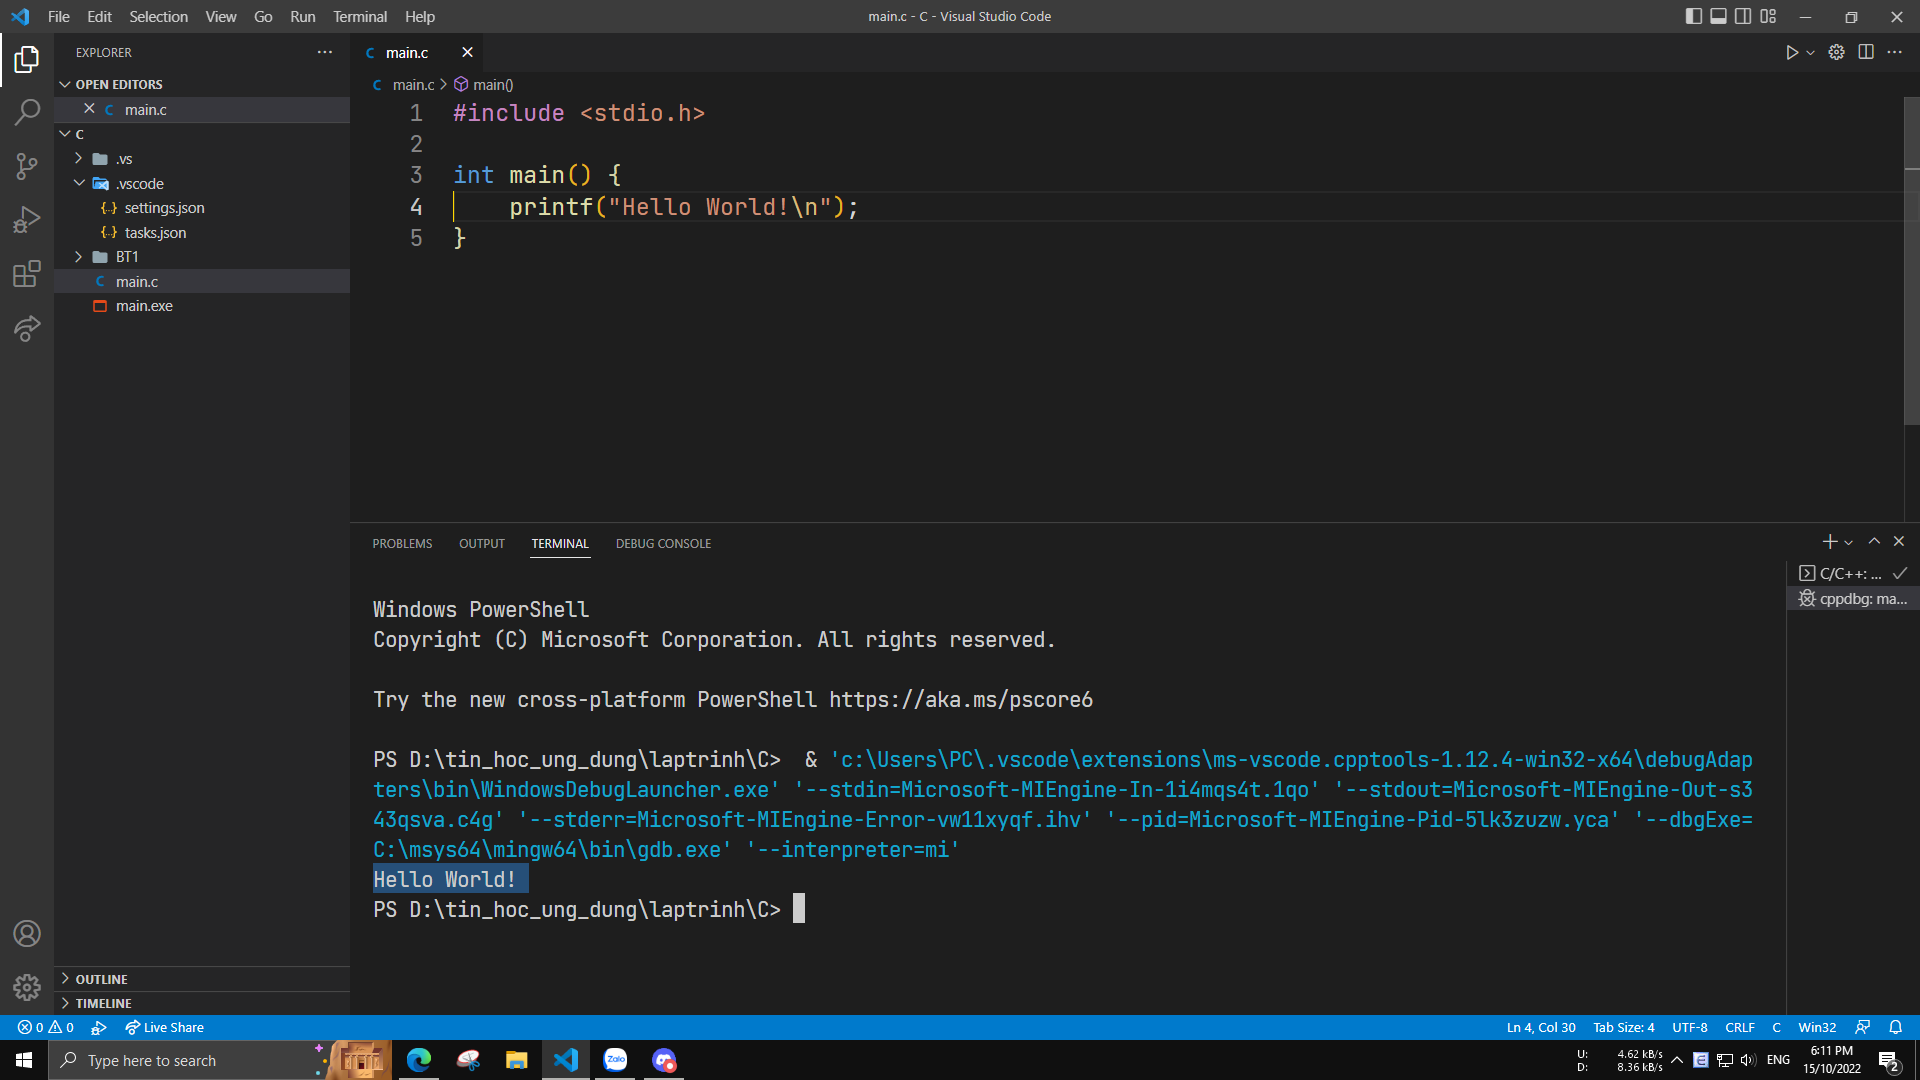
\includegraphics[scale=0.28]{Screenshot_(1346).png}
		\end{center}
		\caption{Bài 1.2 (a)}
	\end{figure}
	\newline
	\begin{figure}[h]
		\begin{center}
			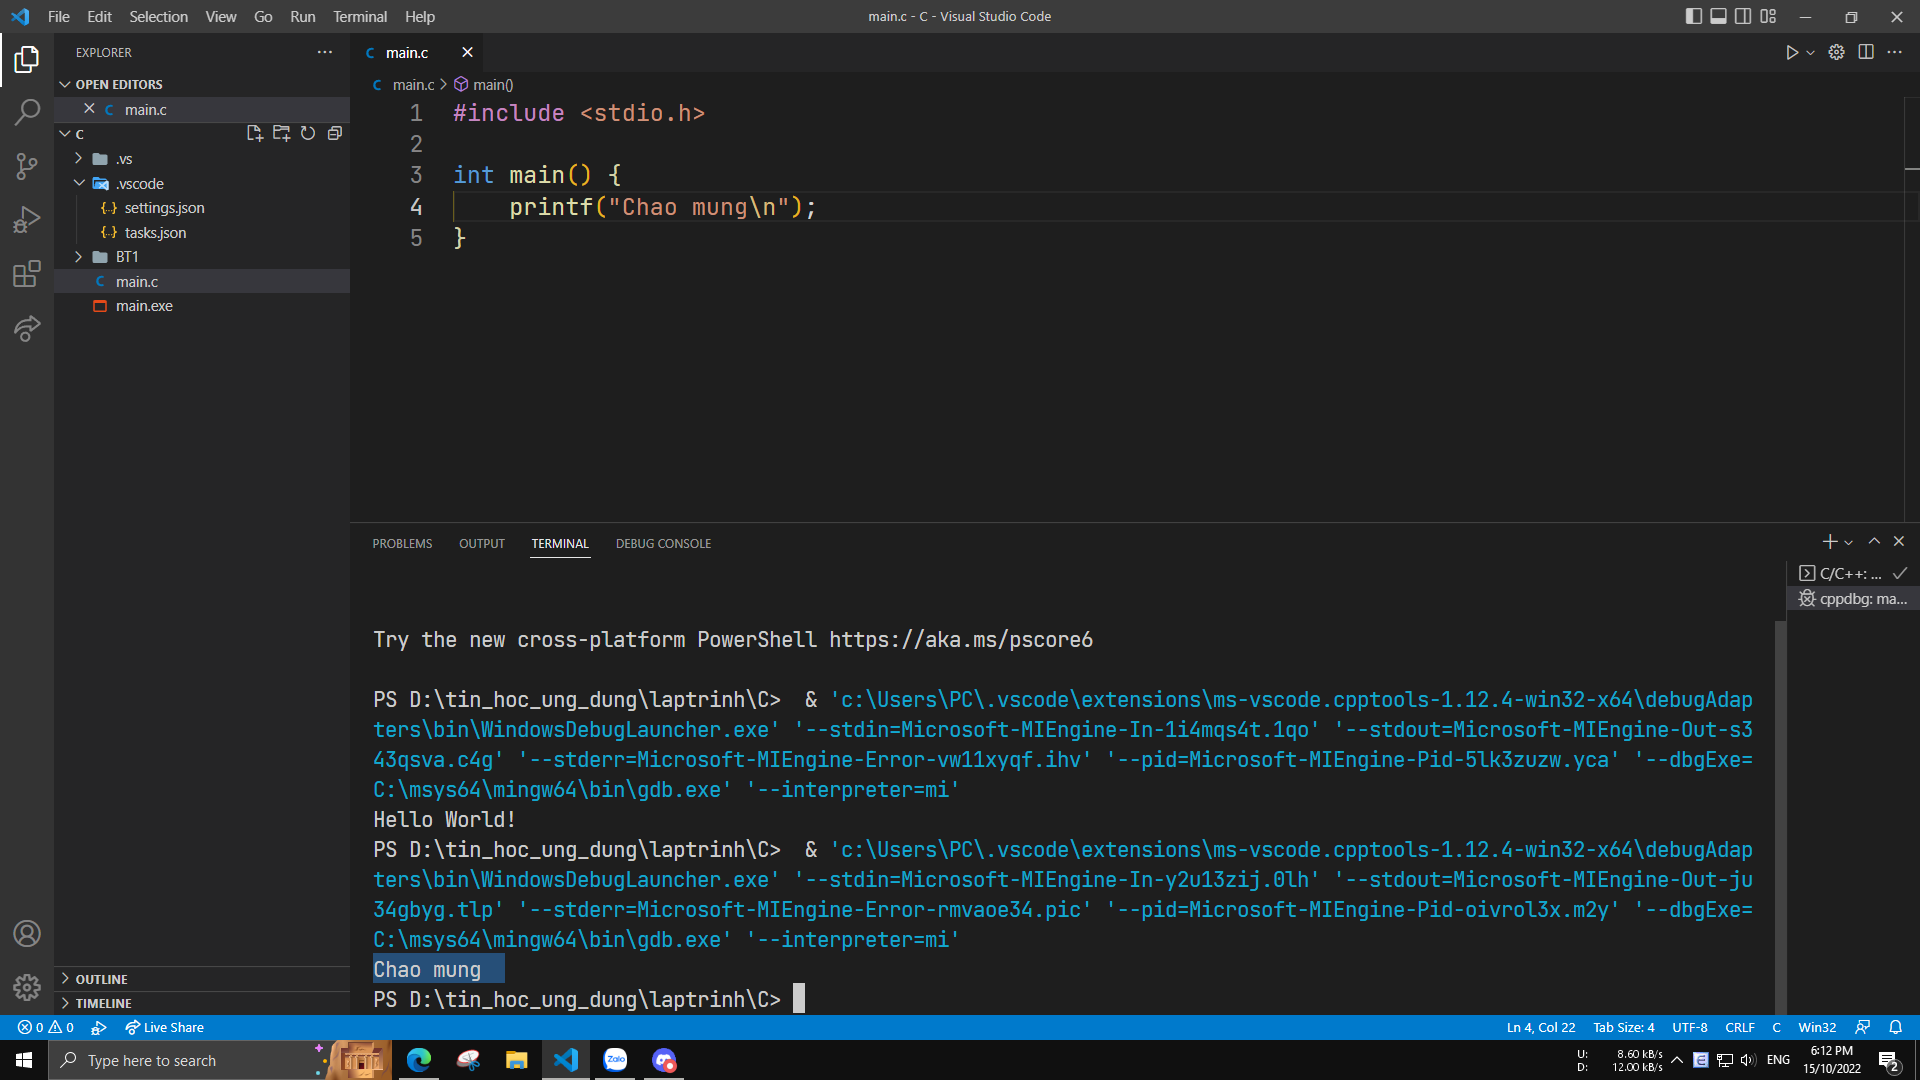
\includegraphics[scale=0.28]{Screenshot_(1347).png}
		\end{center}
		\caption{Bài 1.2 (b)}
		\vspace{1cm}
		\begin{center}
			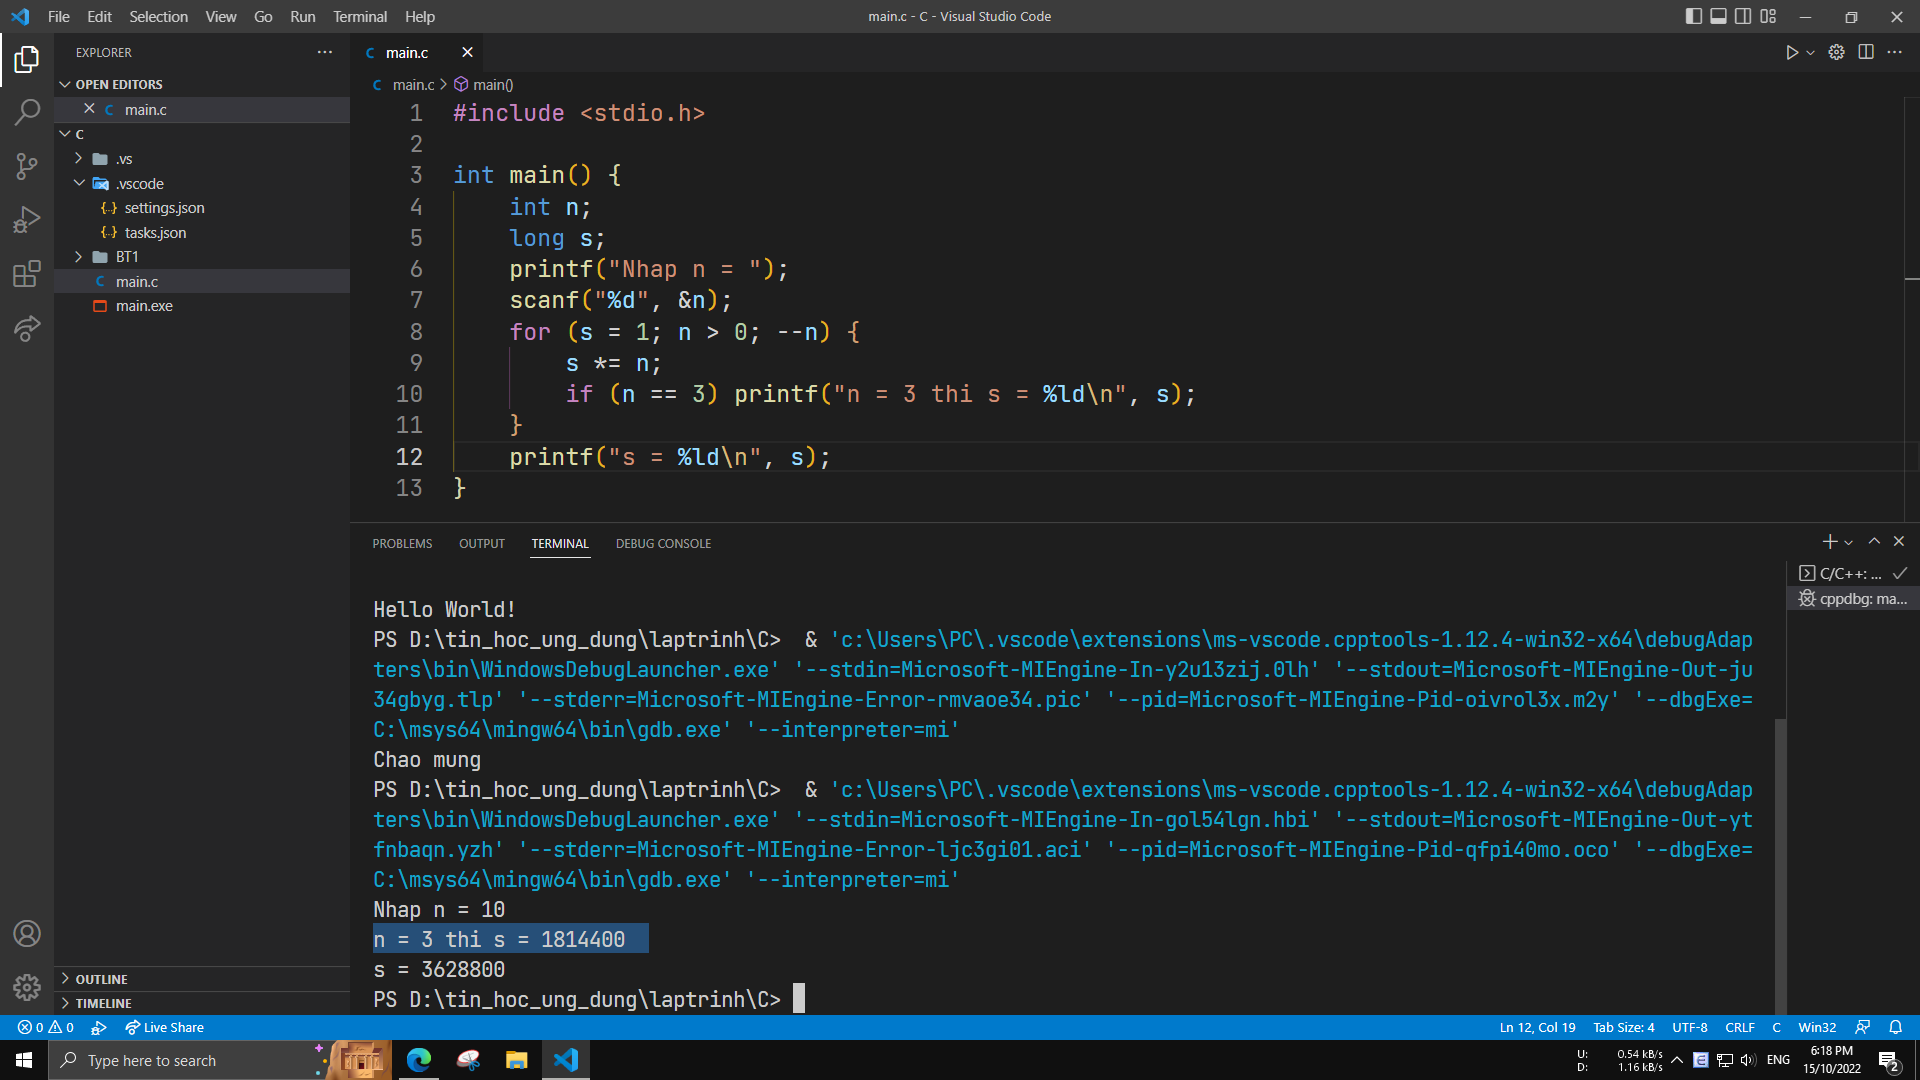
\includegraphics[scale=0.28]{Screenshot_(1348).png}
		\end{center}
		\caption{Bài 1.3}
	\end{figure}
	\begin{figure}[h]
		\begin{center}
			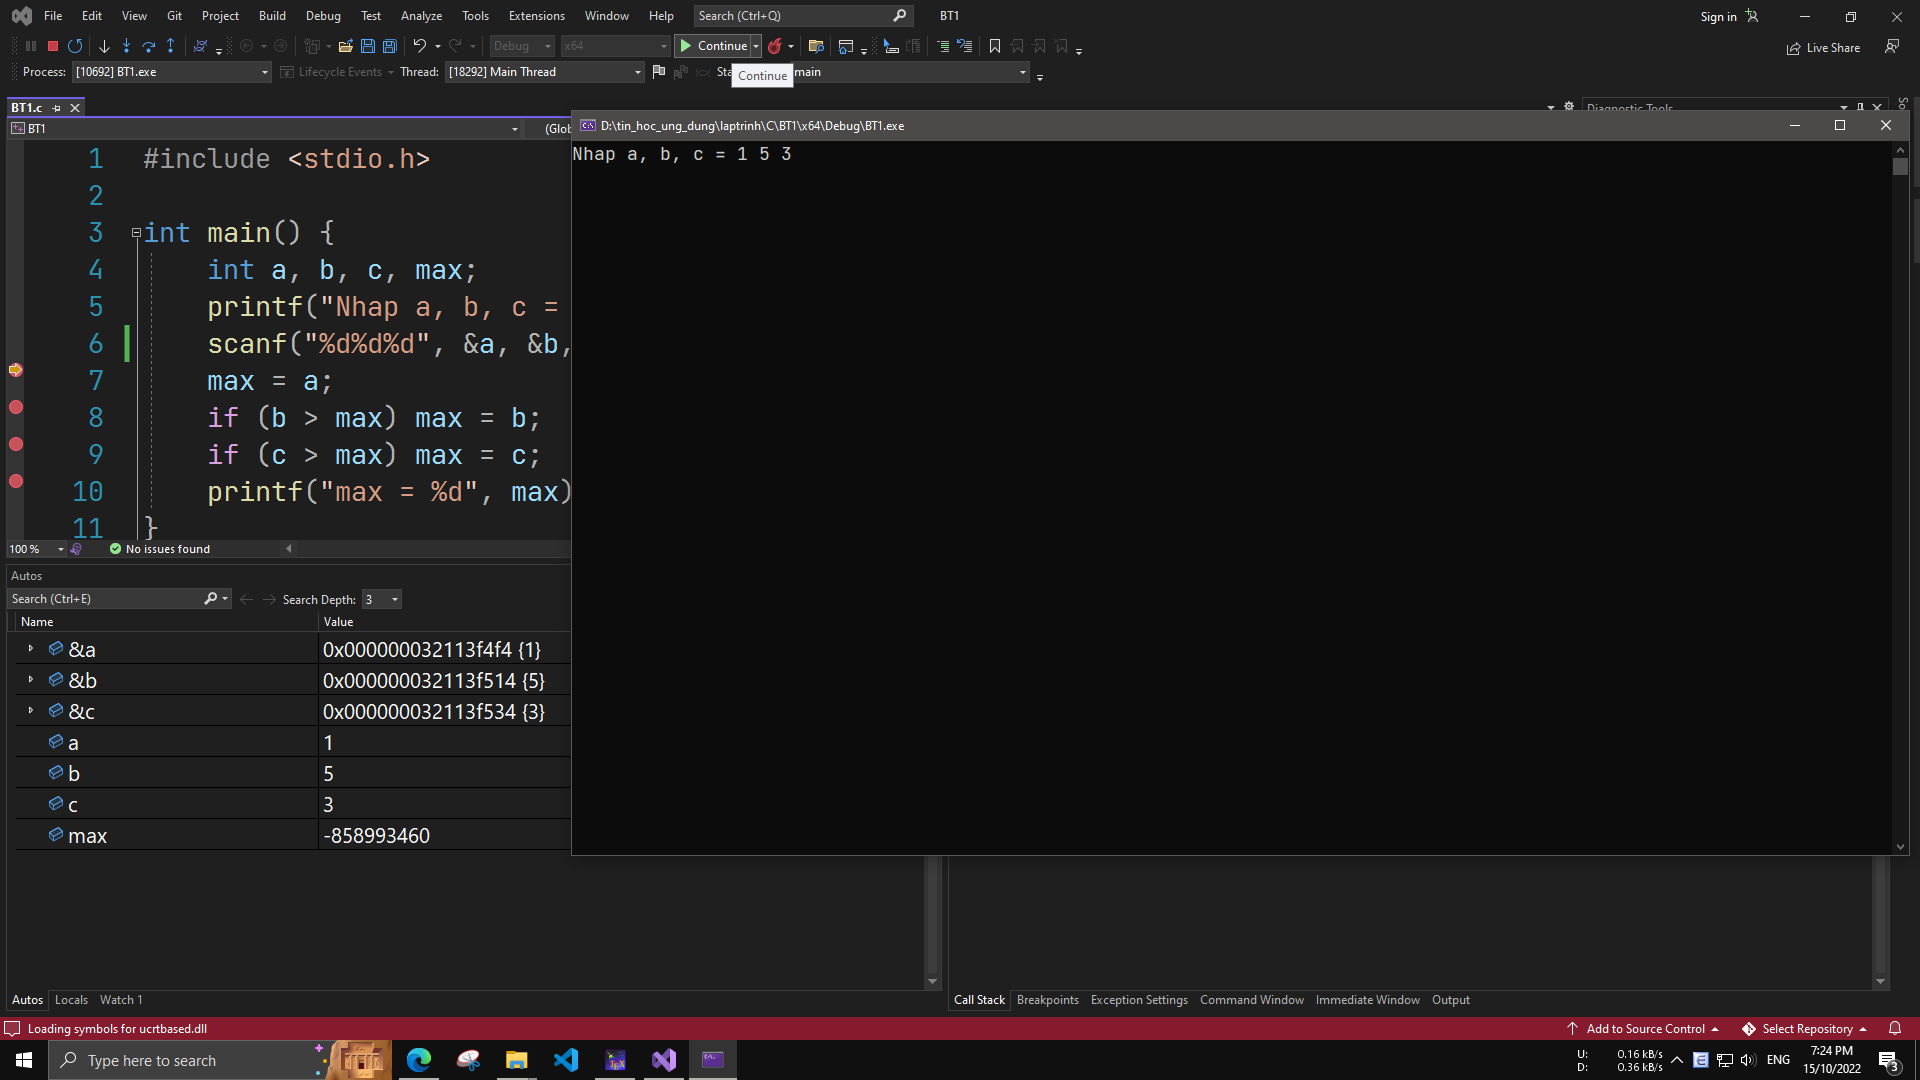
\includegraphics[scale=0.28]{Screenshot (1359).png}
		\end{center}
		\begin{center}
			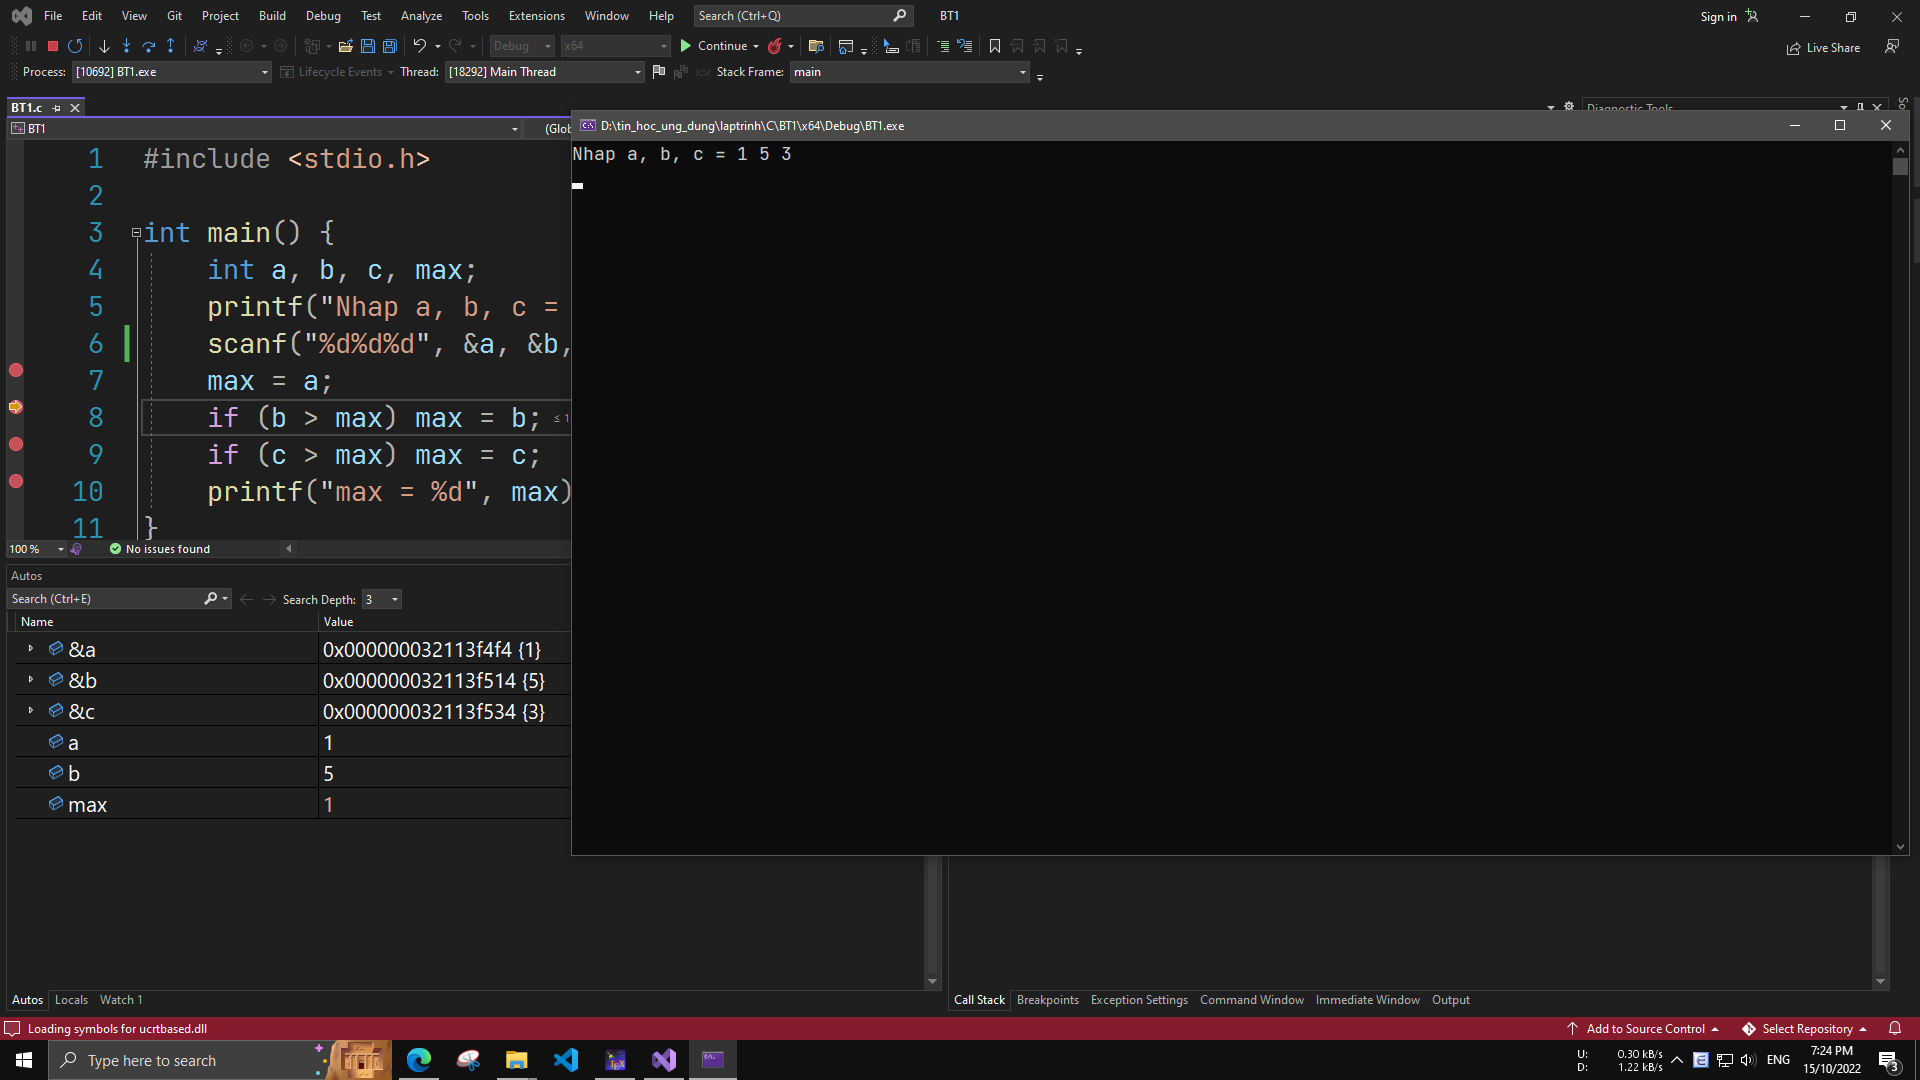
\includegraphics[scale=0.28]{Screenshot (1360).png}
		\end{center}
		\caption{Bài 1.5 (a) (1)}
	\end{figure}
	\begin{figure}[h]
		\begin{center}
			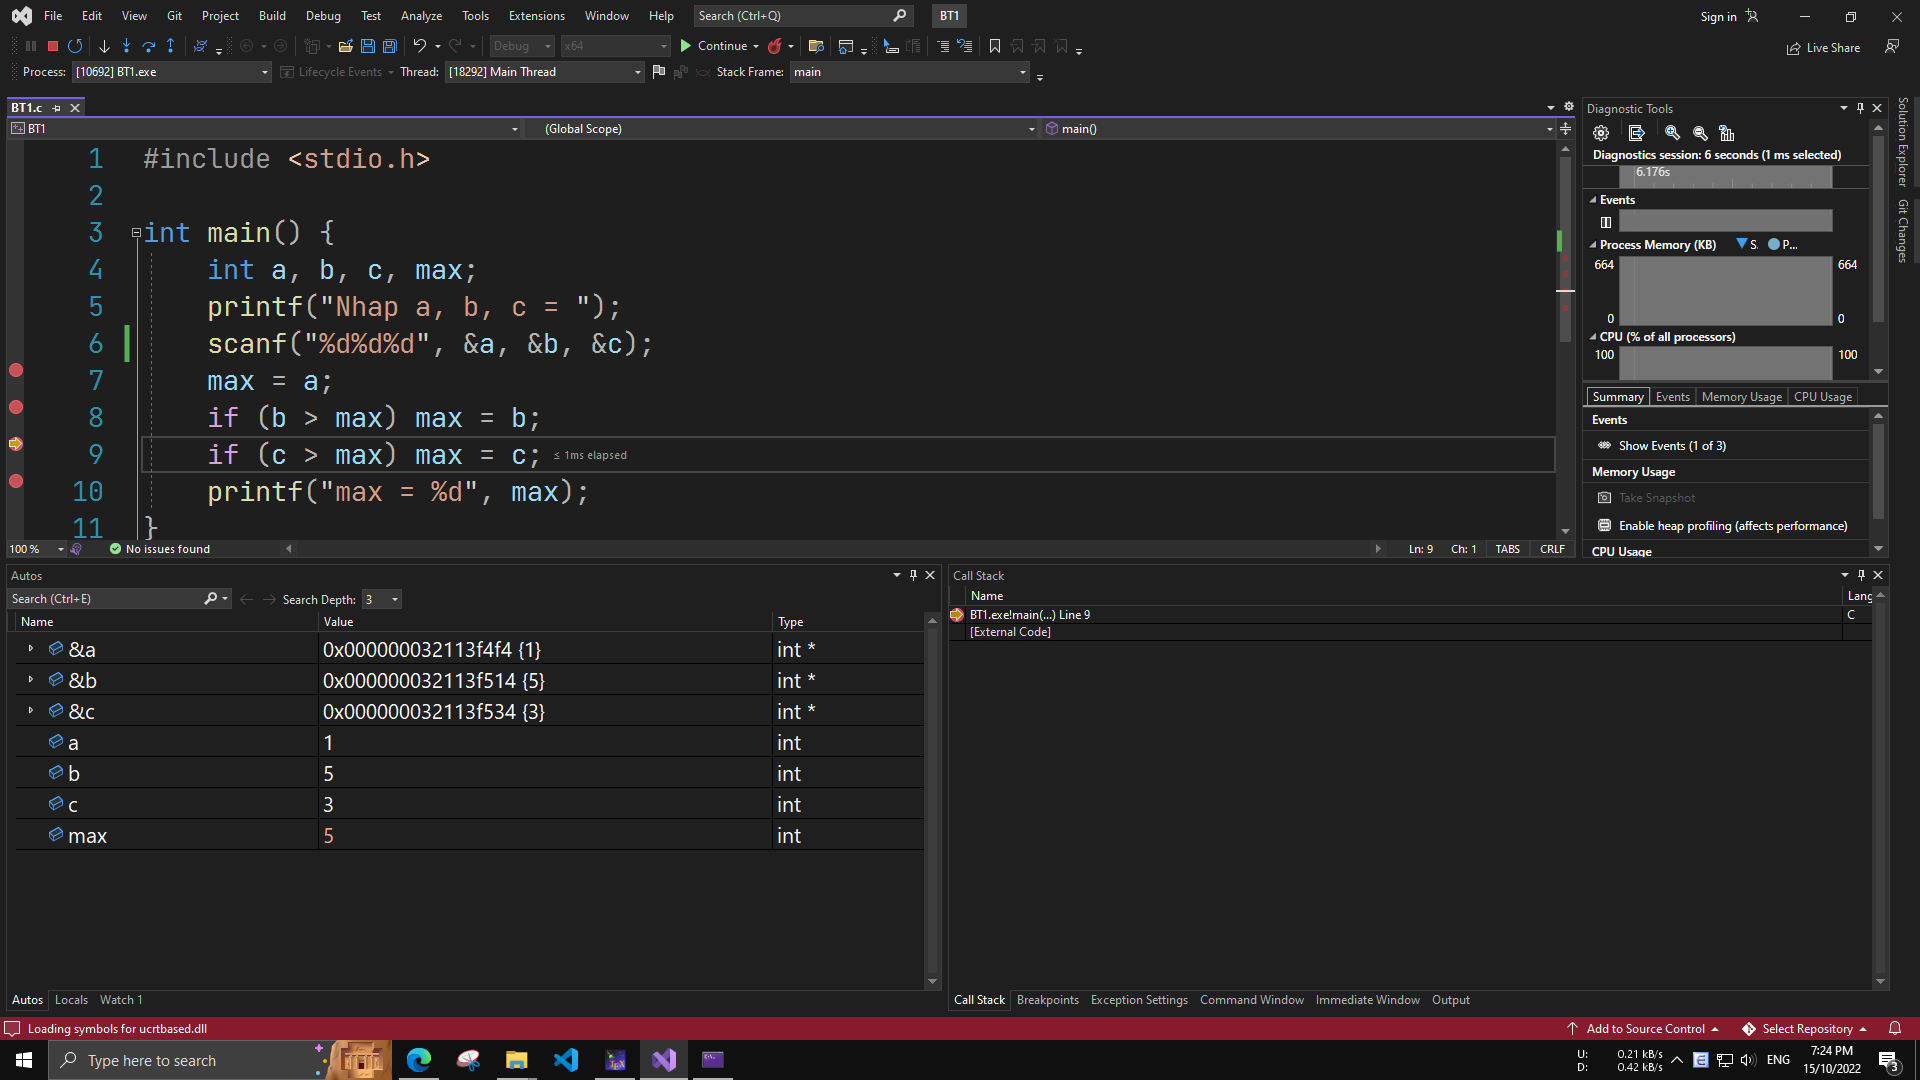
\includegraphics[scale=0.28]{Screenshot (1361).png}
		\end{center}
		\begin{center}
			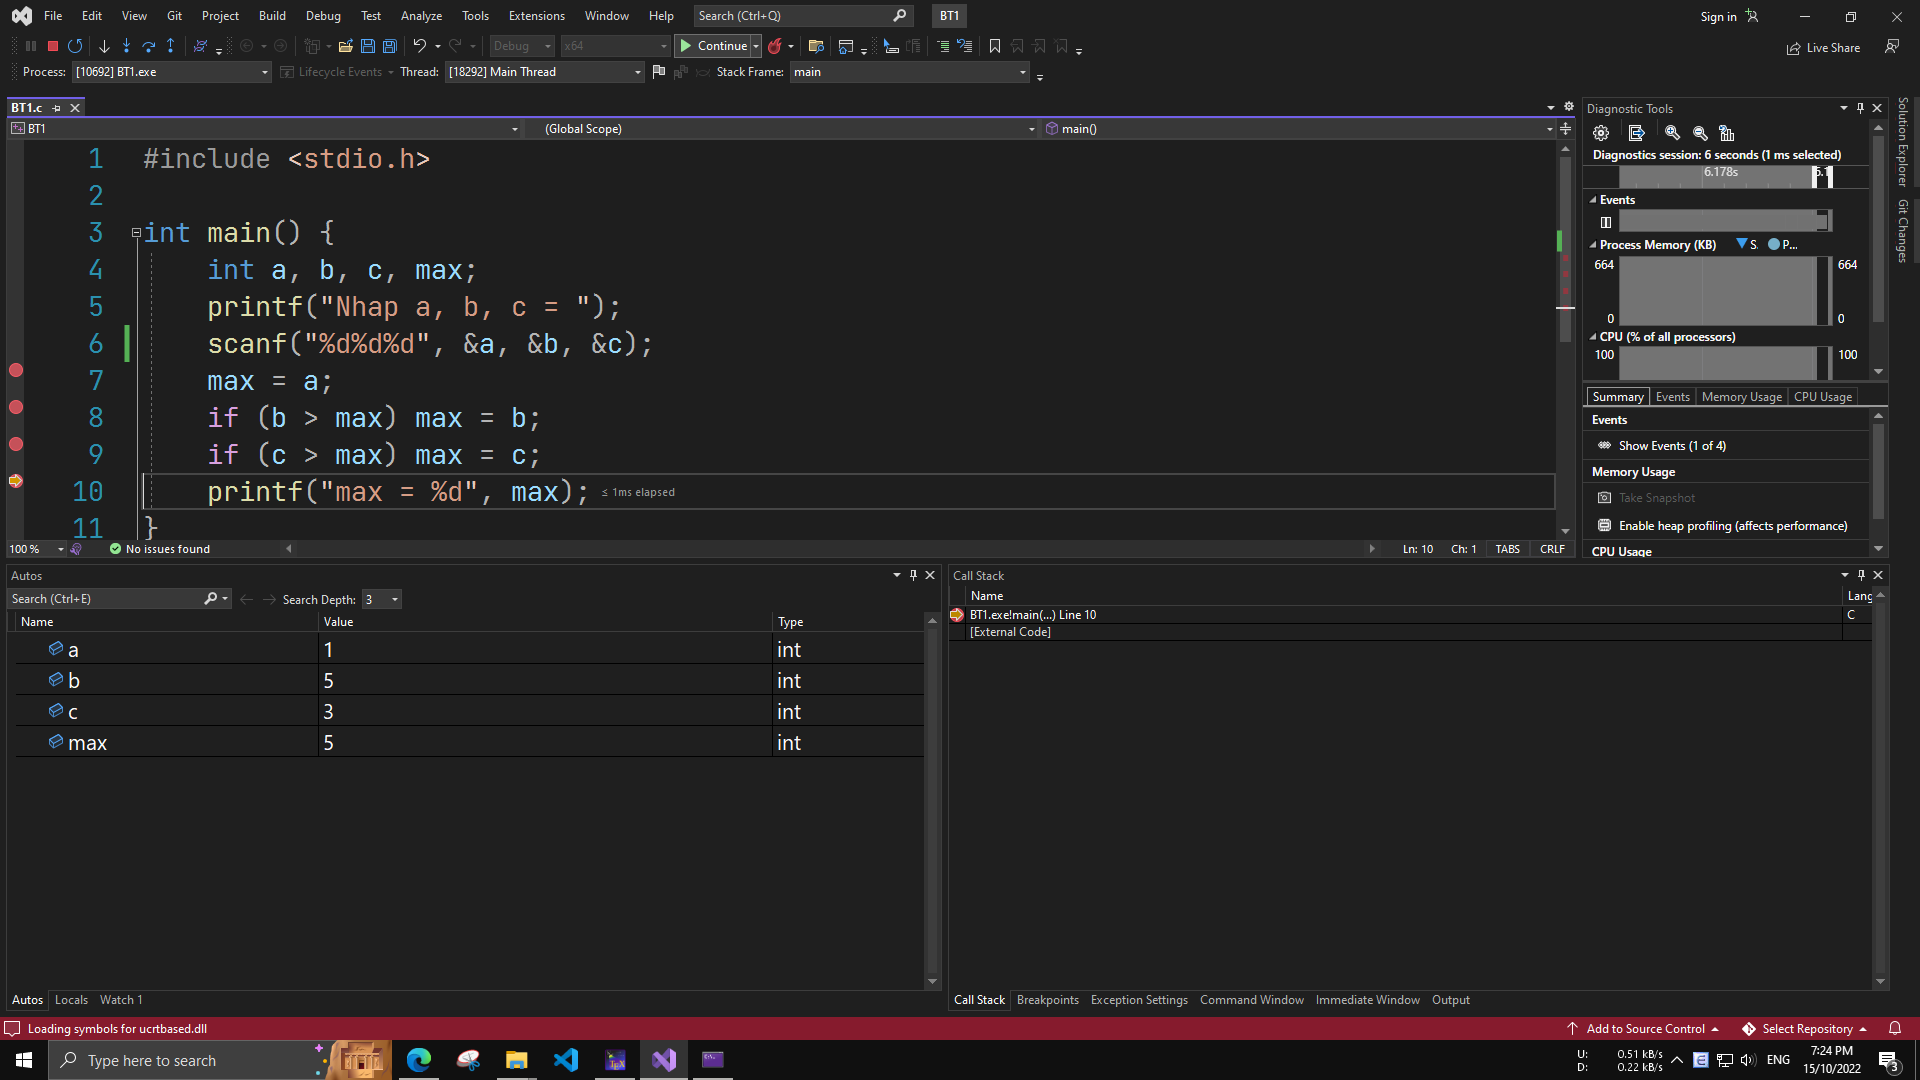
\includegraphics[scale=0.28]{Screenshot (1362).png}
		\end{center}
		\caption{Bài 1.5 (a) (2)}
	\end{figure}
	\begin{figure}[h]
		\begin{center}
			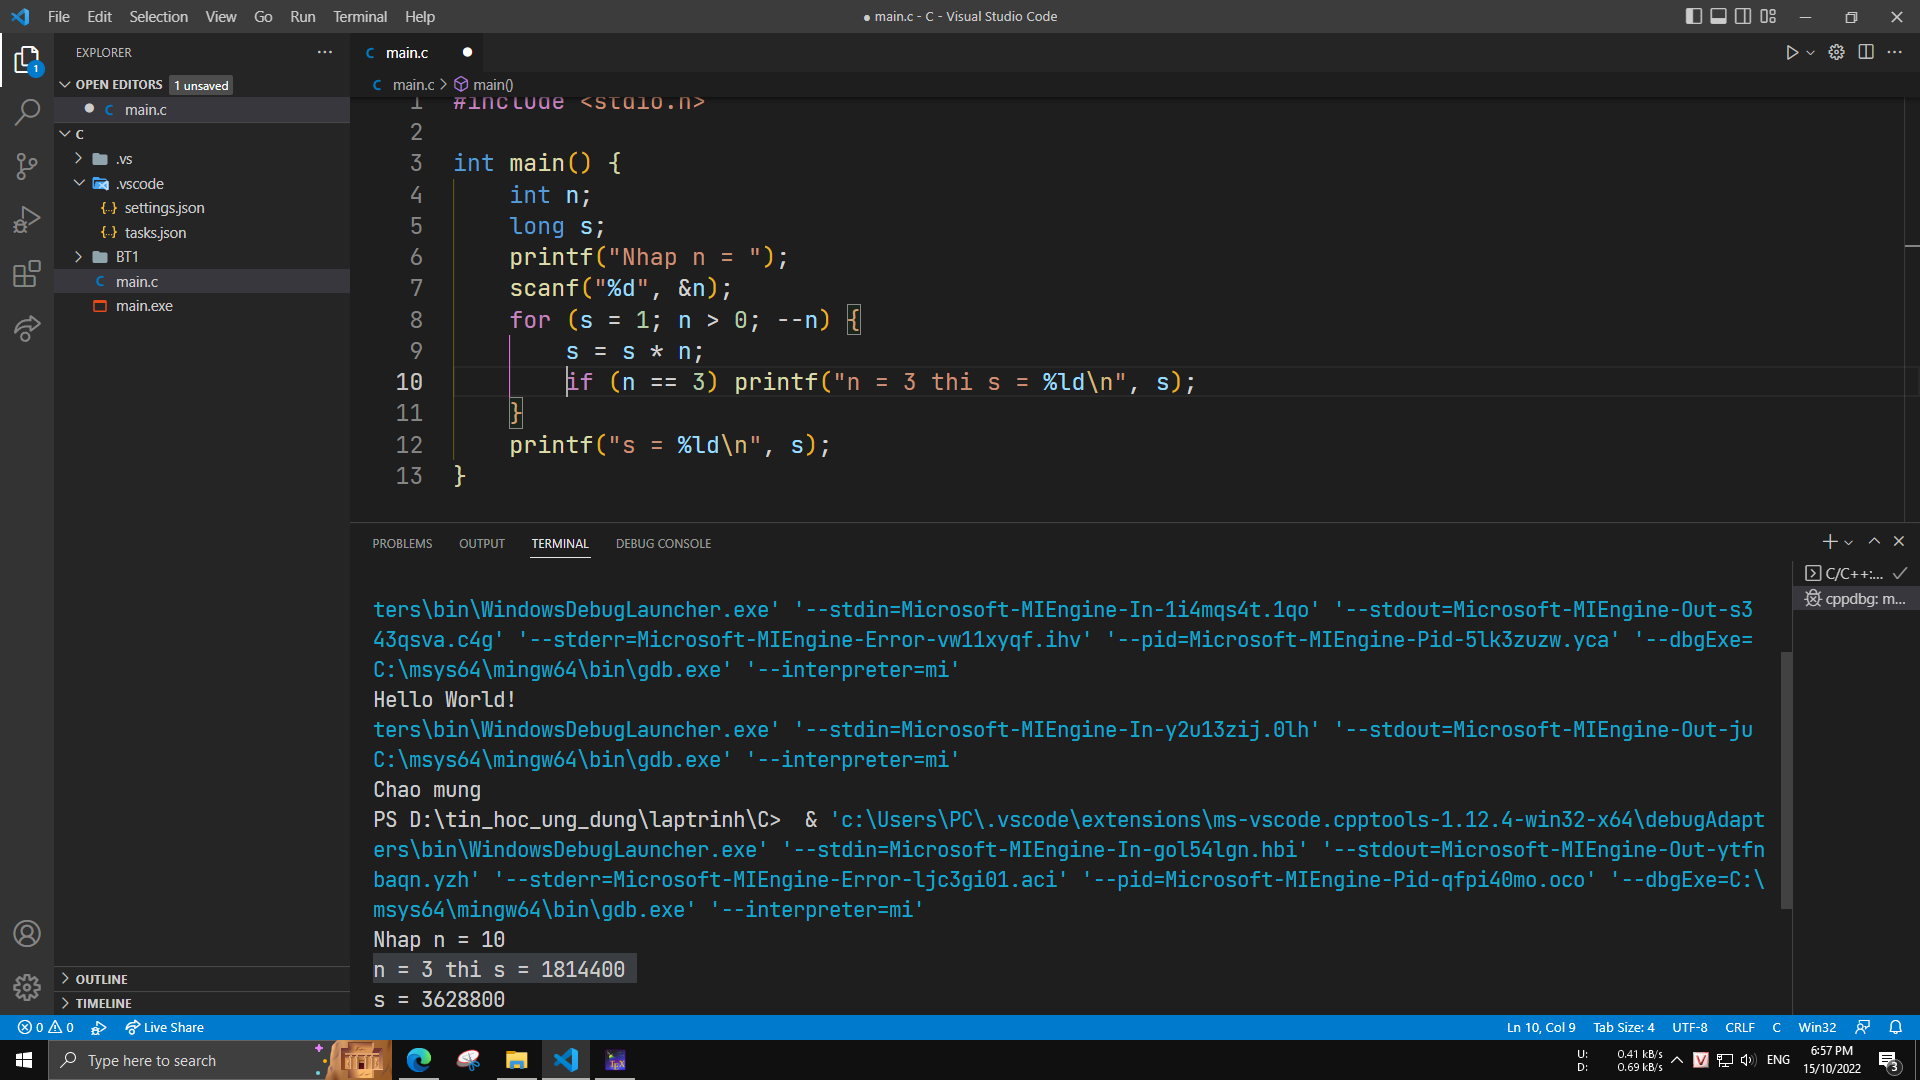
\includegraphics[scale=0.28]{Screenshot_(1349).png}
		\end{center}
		\begin{center}
			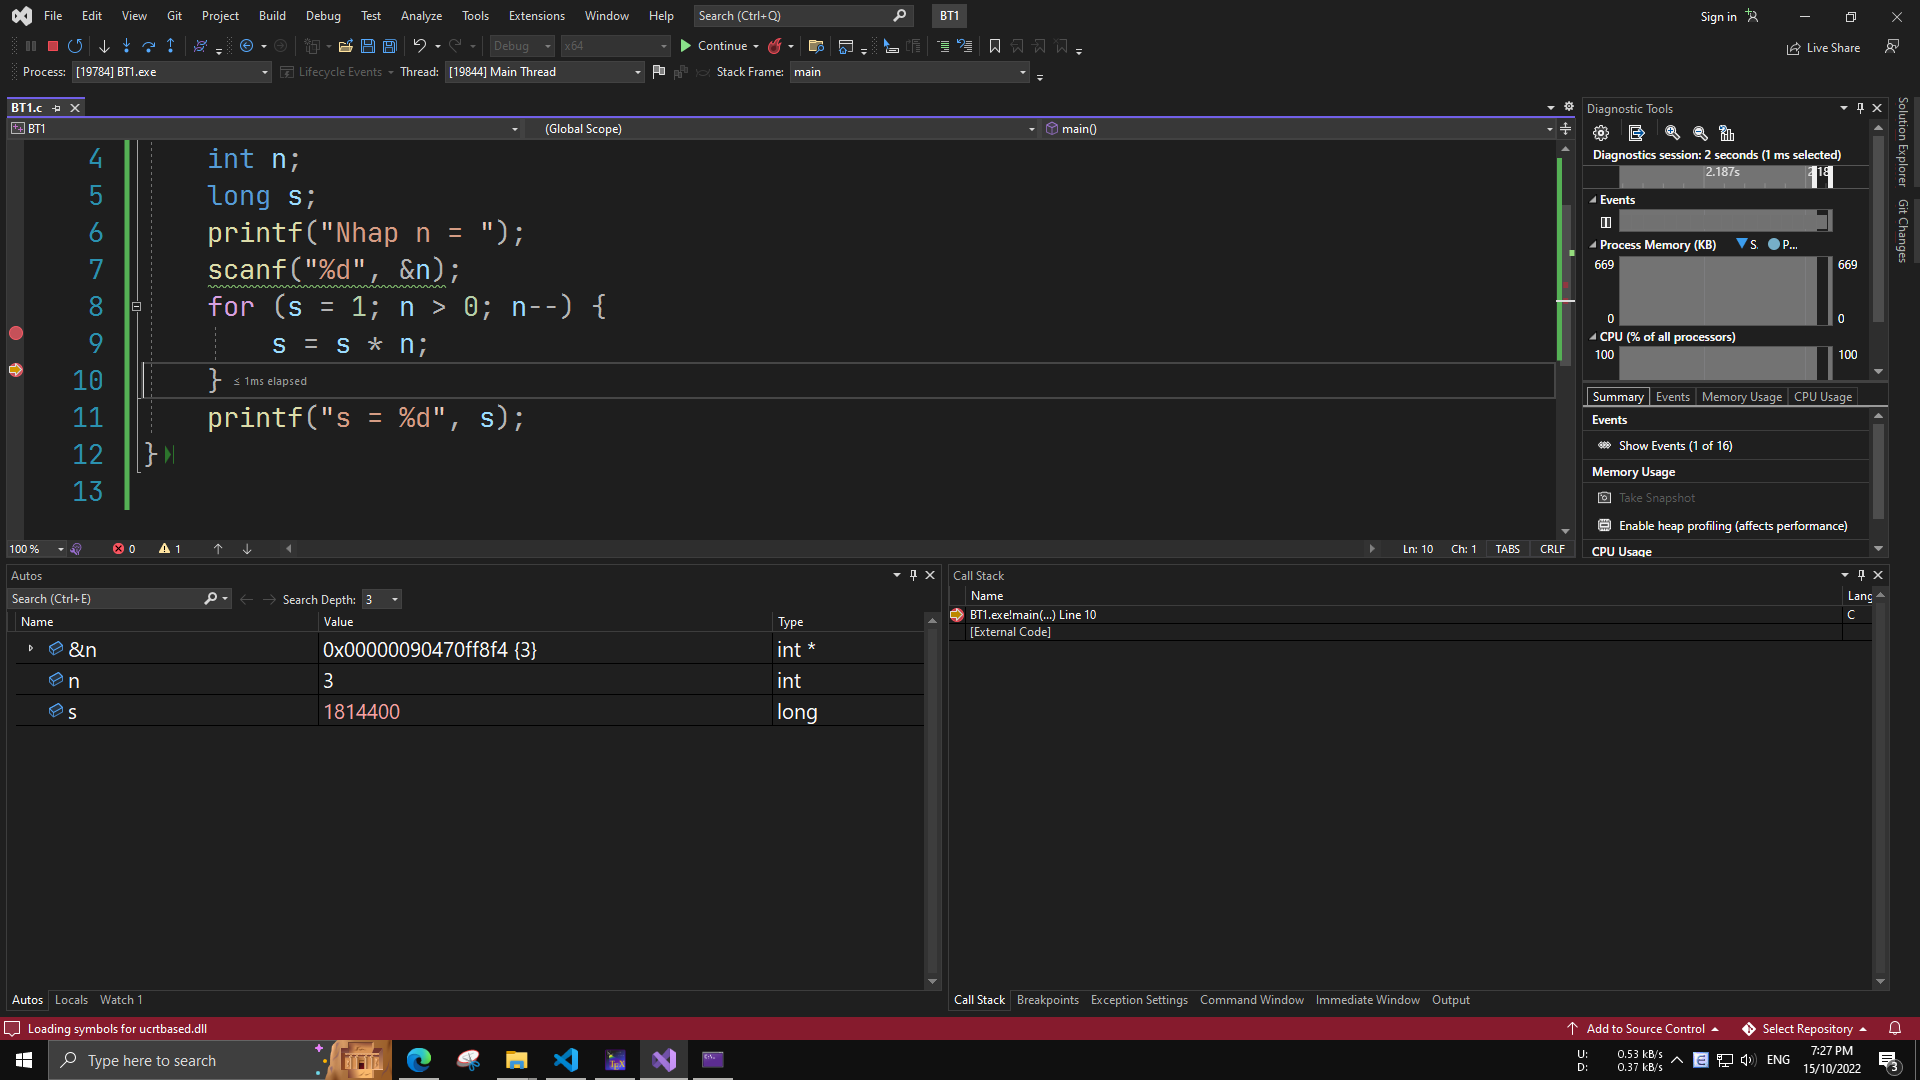
\includegraphics[scale=0.28]{Screenshot (1363).png}
		\end{center}
		\caption{Bài 1.5 (b)}
	\end{figure}

\end{document}